% ============================================================
% T-DOME Paper I: The Seed
% T-DOME three-paper series, Paper I -- October 2026 revision
% ============================================================

\documentclass[12pt]{article}
\usepackage[margin=1in]{geometry}
\usepackage{amsmath,amssymb,amsthm}
\usepackage[hidelinks]{hyperref}
\hypersetup{pdftitle={Memory as a Usable Resource: Correlations, Records and Complete Endpoint Accounting},pdfauthor={Sidong Liu}}
\usepackage{booktabs}
\usepackage{physics}
\usepackage{graphicx}
\usepackage{caption}
\usepackage{array}
\newcolumntype{P}[1]{>{\raggedright\arraybackslash}p{#1}}
\graphicspath{{TDOME_I_supplement/}}

\newtheorem{theorem}{Theorem}
\newtheorem{lemma}[theorem]{Lemma}
\newtheorem{proposition}[theorem]{Proposition}
\newtheorem{definition}[theorem]{Definition}
\newtheorem{remark}[theorem]{Remark}
\newtheorem{corollary}[theorem]{Corollary}
\newtheorem{conjecture}[theorem]{Conjecture}

\title{Memory as a Usable Resource:\\
Correlations, Records and Complete Endpoint Accounting}

\author{Sidong Liu, PhD \\
\small iBioStratix Ltd \\
\small \texttt{sidongliu@hotmail.com}}

\date{Revised October 2026}

\begin{document}
\emergencystretch=2em
\raggedbottom
\hbadness=10000
\vbadness=10000
\maketitle

% ============================================================
\begin{abstract}
A stored correlation has value only through an operation that can use it.
We ask which correlations can fund a free-energy gain, who can read them
and what reading, feedback and memory reset cost. The survival functional
$\mathcal S=\Delta F-W$ obeys an exact balance retaining mutual information,
environmental displacement from equilibrium, control energy and
interaction energy. Three models distinguish their roles: Lorentz--Drude
dephasing has no backflow at any temperature but a nonzero interaction
energy; an autonomous two-qubit recurrence saturates the correlation
budget without a pointer record; fresh-memory collisions create records
available to several readers. A classical memory used for feedback is
worth at most $k_BT I(X{:}M)$, with matched quasistatic feedback approaching the
value. Every feedback protocol assumes a posterior and loses at least
$k_BT$ times its expected divergence from the true posterior. A wrong
readout model can therefore make a record worse than no memory. For a
tail-controlled estimate from $n$ references per sign, calibration has
leading loss $k_BT(1+g^2/(1-b^2))/(4n)$ and pays through reuse. Within a reset menu with no added purity, positive read--harvest--reset
work requires accessible correlated side information. Two partially mixed
record ports realize this possibility: one drives matched feedback and the
other reduces the reset cost through a reversible parity operation. These results establish
the memory--self--introspection route's first functional link: relevant
memory permits a gain, a model of one's readout realizes its full value,
and calibration builds that model at a calculable cost. A separate finite-history
classification bound proves that, for each fixed observation window, a
longer finite episode can improve the attainable decision risk.
\end{abstract}

\medskip
\noindent\textbf{Keywords}: open quantum systems, information thermodynamics, system--environment correlations, quantum records, feedback control, self-calibration, interaction energy, non-Markovian dynamics

% ============================================================
\section{Introduction}
\label{sec:intro}

\subsection{What memory can pay for}

A system coupled to a thermal bath can lose the free energy needed for further action. An autonomous detailed-balance semigroup makes that loss precise; a structured environment can instead return correlations at a later time. Persistent structures, from molecular machines to organisms, maintain themselves by importing low-entropy energy and exporting entropy \cite{Schrodinger1944}. Within that general picture a narrower question can be answered exactly: when can correlations that a system has already built with its environment fund a later interval, and what does it take for an agent to turn a stored record into usable work?

Two errors are easy to make here. One is to treat any memory effect in the reduced dynamics as a resource. A memory kernel represents retained history; it does not guarantee that the history can be used, and the sign of the free-energy balance is fixed by the resources and the endpoint terms, not by Markovianity as such. The other is to treat information as free once it is stored. A record has value only for an agent that can read it, act on it with a correct model of its own reading, and dispose of the memory afterwards; each step has a price. The endpoint balance and the feedback task below specify which terms must be paid.

\subsection{Position within the series}

This paper is the first of the T-DOME (Thermodynamic Dynamics of Observer-Memory Entanglement) series, the third line of a programme whose other two lines are HAFF and Q-RAIF.

\begin{center}
\small
\setlength{\tabcolsep}{4pt}%
\begin{tabular}{@{}lP{3.4cm}cP{4.2cm}@{}}
\toprule
\textbf{Line} & \textbf{Question} & & \textbf{Role here} \\
\midrule
HAFF~\cite{Liu2026HAFF_E,Liu2026HAFF_F}
  & How do stable, public records form?
  & Ocean
  & Supplies the collision model of records \\[3pt]
Q-RAIF~\cite{Liu2026QRAIF_B}
  & How does a subsystem read and act on its world?
  & Fish
  & Reading and control interfaces; costs of persistence \\[3pt]
\textbf{T-DOME I} (this work)
  & What can stored correlations fund, and for whom?
  & Seed
  & Ledger, correlation types, value of memory and readout model \\[3pt]
T-DOME II~\cite{Liu2026TDOME_II}
  & How can a bounded agent organize what it keeps?
  & Ego
  & Frame and feature selection under a budget \\[3pt]
T-DOME III~\cite{Liu2026TDOME_III}
  & How does an agent keep its model of itself calibrated?
  & Loop
  & Detection, tracking and body-gated repair \\
\bottomrule
\end{tabular}
\end{center}

The three T-DOME papers form a conditional sequence of models along what the programme calls the memory--self--introspection route: an agent keeps records of its world, models its own access to that world, and checks that model against references. The present paper supplies the first link and the thermodynamic currency for the other two. It shows in one explicit task that a memory is informationally necessary for a work gain, that every protocol acts on an implied posterior and obtaining the full value requires that posterior to match the agent's readout, and that calibrating the model from references is an achievable mechanism whose cost and benefit can be computed. Paper~II shows that under a reading budget a self-frame formed from records is informationally necessary for the task, prices it and identifies the blind spot it creates; Paper~III develops drift detection, priced tracking and history-selected repair of body-gated access.

\subsection{Results}

\begin{itemize}
\item An exact accounting identity for the survival functional with every endpoint term retained (Theorem~\ref{thm:advantage}), a budget bound and a charge--discharge interval closure (Corollary~\ref{cor:three_regimes}, Proposition~\ref{prop:full_cycle}), and a restricted autonomous ceiling for a detailed-balance semigroup (Theorem~\ref{thm:autonomous_ceiling}).
\item Three exact models with different roles (Section~\ref{sec:models}): no backflow at any temperature and a nonzero interaction-energy term in the Lorentz--Drude pure-dephasing model (Propositions~\ref{prop:ld_monotone} and~\ref{prop:ld_energy}); exact saturation of the correlation budget without any record in an autonomous two-qubit model (Proposition~\ref{prop:two_qubit}); the complete ledger of the collision model of records (Proposition~\ref{prop:collision_ledger}).
\item The work value of a record held in a classical memory and its information-theoretic ceiling (Theorem~\ref{thm:value}); the price of acting on a wrong posterior, which every protocol implicitly assumes (Theorem~\ref{thm:selfmodel}); the local metric of that price and the loss after calibration from references (Proposition~\ref{prop:calibration}), with the resulting amortization rule (Corollary~\ref{cor:amortization}) and a drift law for self-calibration, proved in Paper~III (Proposition~\ref{conj:drift}).
\item A read--harvest--reset bound for a specified reset menu (Proposition~\ref{prop:cycle}), and a two-mixed-port realization with a constructive conditional reset (Proposition~\ref{prop:mixed_task}). The task restores the private memory and the retained record's marginal, not the complete record source.
\end{itemize}
Sections~\ref{sec:arrow}--\ref{sec:numerical} distinguish temporal influence from kernel memory, price specified archives and compare retained history with fixed observation windows.

% ============================================================
\section{Thermodynamic setting}
\label{sec:prelim}

\subsection{Open systems and memory kernels}

Consider $\mathcal H=\mathcal H_S\otimes\mathcal H_E$ with total Hamiltonian
\begin{equation}
\label{eq:H_total}
H(t)=H_S(t)\otimes\mathbb 1_E+\mathbb 1_S\otimes H_E+H_{\mathrm{int}}(t),\qquad H_S(t)=H_R+H_{\mathrm{ctrl}}(t),
\end{equation}
where $H_R$ is the fixed bare system Hamiltonian, $H_{\mathrm{ctrl}}$ the control and $H_{\mathrm{int}}$ the coupling. Under the Born--Markov and secular approximations the reduced dynamics obeys a GKSL equation \cite{Lindblad1976,GKS1976}. For a fixed environmental reference $\sigma_E$, set $\mathcal P A=\tr_E(A)\otimes\sigma_E$, $\mathcal Q=\mathrm{id}-\mathcal P$ and $\mathcal L(t)A=-i[H(t),A]$. Eliminating the $\mathcal Q$ component gives the exact Nakajima--Zwanzig equation
\begin{equation}
\label{eq:NZ}
\dot\rho_S(t)=-i[H_{\mathrm{eff}}(t),\rho_S(t)]+\int_0^tds\;\mathcal K(t,s)\,\rho_S(s)+\mathcal I_0(t),
\end{equation}
where $H_{\mathrm{eff}}(t)=H_S(t)+\tr_E[H_{\mathrm{int}}(t)(\mathbb 1_S\otimes\sigma_E)]$ and
\[
 \mathcal K(t,s)A=\tr_E\!\left[\mathcal L(t)\mathcal G_Q(t,s)
       \mathcal Q\mathcal L(s)(A\otimes\sigma_E)\right],\qquad
 \mathcal I_0(t)=\tr_E\!\left[\mathcal L(t)\mathcal G_Q(t,0)
       \mathcal Q\rho_{SE}(0)\right].
\]
Here $\mathcal G_Q$ propagates the $\mathcal Q$ subspace with generator $\mathcal Q\mathcal L(t)\mathcal Q$ \cite{Nakajima1958,Zwanzig1960}. The inhomogeneous term vanishes for $\rho_{SE}(0)=\rho_S(0)\otimes\sigma_E$; correlated inputs allowed below generally retain it. Non-Markovian dynamics can show information backflow, a temporary increase of the trace distance between two evolving states \cite{BreuerLainePiilo2009}. Neither the kernel nor backflow is used as a resource below; the accounting identity applies directly to the joint unitary dynamics.

\subsection{Conventions}
\label{subsec:thermo}

\begin{definition}[Thermodynamic setup]
\label{def:thermo_setup}
Let $\beta=(k_BT)^{-1}$. The reference state of the system is $\rho_{\mathrm{eq}}=e^{-\beta H_R}/Z_R$, and its nonequilibrium free energy is
\begin{equation}
\label{eq:F_neq}
F(\rho)=\tr(\rho H_R)-\beta^{-1}S(\rho),\qquad
D(\rho\Vert\rho_{\mathrm{eq}})=\beta\bigl(F(\rho)-F_{\mathrm{eq}}\bigr)\ge0 .
\end{equation}
The environmental reference is the fixed Gibbs state $\rho_E^{\mathrm{th}}=e^{-\beta H_E}/Z_E$. The inclusive work over $[0,\tau]$ is $W=\int_0^\tau\tr\bigl(\rho(t)\,\partial_tH(t)\bigr)dt$, so that $W=\Delta\langle H\rangle$ exactly.
\end{definition}

\begin{definition}[Standing assumptions]
\label{def:assumptions}
Unless stated otherwise:
\begin{enumerate}
\item[\textup{(A1)}] $\mathcal H_S\otimes\mathcal H_E$ is finite dimensional and the total evolution is unitary, generated by \eqref{eq:H_total}. Infinite baths are treated as limits of finite mode sets in which the quantities below have finite limits.
\item[\textup{(A2)}] Every energy change is booked: $W=\Delta\langle H_R\rangle+\Delta\langle H_{\mathrm{ctrl}}\rangle+\Delta\langle H_E\rangle+\Delta\langle H_{\mathrm{int}}\rangle$. Dropping $\Delta\langle H_{\mathrm{int}}\rangle$ is a declared approximation, never a consequence of autonomy.
\item[\textup{(A3)}] $H_E$ is time independent; the actual initial state of the environment need not be $\rho_E^{\mathrm{th}}$.
\item[\textup{(A4)}] The initial state $\rho_{SE}(0)$ may be correlated.
\item[\textup{(A5)}] Relative entropies are finite (full rank, or restriction to supports).
\end{enumerate}
\end{definition}

\subsection{The survival functional}
\label{subsec:survival}

\begin{definition}[Survival functional]
\label{def:survival}
For an interval $[a,b]$,
\begin{equation}
\label{eq:survival}
\mathcal S[a,b]:=F(\rho_S(b))-F(\rho_S(a))-W[a,b],\qquad
\beta\,\mathcal S=-\Sigma,\quad \Sigma:=\beta(W-\Delta F).
\end{equation}
\end{definition}

The name records the intended use: $\mathcal S>0$ means the system gained more free energy than the external protocol invested, a thermodynamic profit; $\mathcal S<0$ means it paid more than it gained. Mathematically $\mathcal S$ is a generalized entropy-balance functional. For an uncorrelated thermal initial environment and zero changes in the endpoint control and interaction energies, $\Sigma\ge0$ and $\mathcal S\le0$. When those endpoint terms change, their signs enter the balance of Theorem~\ref{thm:advantage}. For correlated initial conditions $\Sigma$ can be negative \cite{EspositoLindenbergVandenBroeck2010}, and the next sections say what pays for it.

In measurement-based feedback, the generalized second law $\Sigma\ge-I_{\mathrm{fb}}$ allows $\mathcal S>0$ at the expense of the information $I_{\mathrm{fb}}$ gained by measurement \cite{SagawaUeda2008,SagawaUeda2010,SagawaUeda2012}. Pre-existing correlations enter the balance in an analogous role. A memory kernel is not itself a measurement record, and the two protocols are kept distinct; Section~\ref{sec:value} returns to feedback with an explicit record.

% ============================================================
\section{A restricted autonomous baseline}
\label{sec:ceiling}

\begin{definition}[Autonomous Davies baseline]
\label{def:autonomous_davies}
The autonomous baseline has $H_{\mathrm{ctrl}}=0$, fixed $H_R$, and a time-independent GKSL generator $\mathcal L$ obtained as the weak-coupling limit of coupling to one thermal bath, satisfying quantum detailed balance with respect to the faithful Gibbs state $\rho_{\mathrm{eq}}$ \cite{Spohn1978,BreuerPetruccione2002}. No measurement, feedback or initial system--bath resource is included.
\end{definition}

\begin{lemma}[Spohn~\cite{Spohn1978}]
\label{lem:spohn}
For a GKSL semigroup $\Lambda_t=e^{\mathcal Lt}$ with invariant state $\rho_{\mathrm{eq}}$, $t\mapsto D(\Lambda_t\rho\Vert\rho_{\mathrm{eq}})$ is nonincreasing.
\end{lemma}

\begin{proof}
Relative entropy is contractive under CPTP maps and $\Lambda_t\rho_{\mathrm{eq}}=\rho_{\mathrm{eq}}$.
\end{proof}

\begin{theorem}[Restricted autonomous ceiling]
\label{thm:autonomous_ceiling}
Under Definition~\ref{def:autonomous_davies}, $\mathcal S[0,\tau]=F(\rho(\tau))-F(\rho(0))\le0$.
\end{theorem}

\begin{proof}
$W=0$, and by \eqref{eq:F_neq} and Lemma~\ref{lem:spohn}, $\beta\Delta F=\Delta D(\rho\Vert\rho_{\mathrm{eq}})\le0$.
\end{proof}

The theorem is a free-energy monotonicity statement for one autonomous detailed-balance class. It is not a ceiling for driven or feedback-controlled Markovian agents, which can persist under continuous driving; time-dependent protocols need an instantaneous detailed-balance hypothesis and a different theorem. The reduced semigroup omits explicit inter-epoch correlations, which is a modelling loss, not a proof that such correlations are unusable.

% ============================================================
\section{Initial-correlation accounting}
\label{sec:advantage}

\subsection{The identity}

The quantum mutual information $I(S{:}E)=S(\rho_S)+S(\rho_E)-S(\rho_{SE})=D(\rho_{SE}\Vert\rho_S\otimes\rho_E)$ measures all correlations between system and environment. For any full-rank $\sigma_E$,
\begin{equation}
\label{eq:chain_general}
D(\rho_{SE}\Vert\rho_S\otimes\sigma_E)=I(S{:}E)+D(\rho_E\Vert\sigma_E),
\end{equation}
an algebraic identity that holds for correlated $\rho_{SE}$ \cite{Wilde2017}.

\begin{lemma}[Information--thermodynamic identity]
\label{lem:info_thermo}
For unitary evolution from any initial state,
\begin{equation}
\label{eq:info_thermo}
\Delta I(S{:}E)+\Delta D(\rho_E\Vert\rho_E^{\mathrm{th}})=\Delta S_S+\beta\,\Delta\langle H_E\rangle .
\end{equation}
\end{lemma}

\begin{proof}
By \eqref{eq:chain_general} with $\sigma_E=\rho_E^{\mathrm{th}}$ and $\ln\rho_E^{\mathrm{th}}=-\beta H_E-\ln Z_E$, the quantity $I+D(\rho_E\Vert\rho_E^{\mathrm{th}})$ equals $-S(\rho_{SE})+S(\rho_S)+\beta\langle H_E\rangle+\ln Z_E$. Unitarity keeps $S(\rho_{SE})$ fixed, and taking differences gives \eqref{eq:info_thermo}.
\end{proof}

\begin{theorem}[Survival balance]
\label{thm:advantage}
Under \textup{(A1)--(A5)}, for any interval and any initial state,
\begin{equation}
\label{eq:advantage}
\boxed{\;
\beta\,\mathcal S=-\Delta I(S{:}E)-\Delta D(\rho_E\Vert\rho_E^{\mathrm{th}})
-\beta\,\Delta\langle H_{\mathrm{ctrl}}\rangle-\beta\,\Delta\langle H_{\mathrm{int}}\rangle .\;}
\end{equation}
\end{theorem}

\begin{proof}
By (A2) and $\Delta F=\Delta\langle H_R\rangle-\beta^{-1}\Delta S_S$,
$\Sigma=\beta(W-\Delta\langle H_R\rangle)+\Delta S_S=(\Delta S_S+\beta\Delta\langle H_E\rangle)+\beta\Delta\langle H_{\mathrm{ctrl}}\rangle+\beta\Delta\langle H_{\mathrm{int}}\rangle$. Lemma~\ref{lem:info_thermo} replaces the bracket by $\Delta I+\Delta D$, and $\beta\mathcal S=-\Sigma$.
\end{proof}

The identity is exact. It is the Esposito--Lindenberg--Van den Broeck decomposition \cite{EspositoLindenbergVandenBroeck2010} written with arbitrary initial correlations and with both endpoint terms kept. It is dynamics-agnostic: Markovianity does not enter, and a memory kernel matters only if a model shows that it preserves correlations across an interval boundary and later allows their consumption. Autonomy removes the control term but not the interaction term; Section~\ref{subsec:ld} gives an autonomous model in which the interaction energy changes at every time.

\subsection{Regimes and the budget}

\begin{corollary}[Regimes and budget]
\label{cor:three_regimes}
Suppose $\Delta\langle H_{\mathrm{ctrl}}\rangle=\Delta\langle H_{\mathrm{int}}\rangle=0$ on the interval, as for a switched protocol whose control and interaction Hamiltonians are zero at both endpoints.
\begin{enumerate}
\item If the interval starts from a product state with a thermal environment, $\beta\mathcal S=-I(S{:}E;b)-D(\rho_E(b)\Vert\rho_E^{\mathrm{th}})\le0$.
\item If correlations are consumed, $\Delta I<0$, and $|\Delta I|>\Delta D(\rho_E\Vert\rho_E^{\mathrm{th}})$, then $\mathcal S>0$.
\item In every case $\beta\mathcal S[a,b]\le I(S{:}E;a)+D(\rho_E(a)\Vert\rho_E^{\mathrm{th}})$.
\end{enumerate}
\end{corollary}

\begin{proof}
Insert the hypotheses into \eqref{eq:advantage} and use $I\ge0$, $D\ge0$ at the end of the interval.
\end{proof}

When the endpoint terms do not vanish they are added to the budget with their signs. The budget in (iii) is the profit ceiling: correlations present at the start of the interval plus the environment's displacement from equilibrium.

\begin{proposition}[Charge--discharge interval closure]
\label{prop:full_cycle}
Under the hypotheses of Corollary~\ref{cor:three_regimes} at the times $0$, $t^*$ and $\tau$, and with $I(S{:}E;0)=0$ and $\rho_E(0)=\rho_E^{\mathrm{th}}$,
\begin{align*}
\beta\mathcal S[0,t^*]&=-I(t^*)-D(t^*)\le0,\\
\beta\mathcal S[t^*,\tau]&=-[I(\tau)-I(t^*)]-[D(\tau)-D(t^*)],\\
\beta\mathcal S[0,\tau]&=-I(\tau)-D(\tau)\le0,
\end{align*}
with $D(t)=D(\rho_E(t)\Vert\rho_E^{\mathrm{th}})$.
\end{proposition}

\begin{proof}
$\Delta F$ and $W$ are additive over concatenated intervals, and Theorem~\ref{thm:advantage} applies to each interval.
\end{proof}

A positive second interval is funded by the correlations built in the first, and their concatenation cannot have positive $\mathcal S$. No restoration of the complete joint state is assumed in this accounting statement. This charge--discharge structure is realized exactly by the two-qubit model of Section~\ref{subsec:two_qubit}. Under the Born approximation every step restarts from a product state, so the resource is removed by construction; a reduced semigroup law by itself does not say that every microscopic dilation is uncorrelated. BLP backflow and correlation consumption can coincide in particular models, but neither implies the other in general \cite{RivasHuelgaPlenio2014}, so backflow is not a witness for the sign of $\mathcal S$ without the full balance.

% ============================================================
\section{Which correlations can be used: three exact models}
\label{sec:models}

\subsection{Pure dephasing with a Lorentz--Drude bath: no backflow, nonzero interaction energy}
\label{subsec:ld}

Let $\hbar=1$ and
\begin{equation}
\label{eq:ld_model}
H=\frac{\omega_0}2\sigma_z+\sum_k\omega_kb_k^\dagger b_k+\sigma_z\sum_k(g_kb_k+g_k^*b_k^\dagger),\qquad
J(\omega)=\sum_k|g_k|^2\delta(\omega-\omega_k)=\frac{2\lambda\gamma\omega}{\omega^2+\gamma^2},
\end{equation}
with $\lambda,\gamma>0$. With this normalization $\int_0^\infty J(\omega)\omega^{-1}d\omega=\pi\lambda$. The initial state is any system state times the thermal state of the bare bath at inverse temperature $\beta\in(0,\infty]$. Removing the free rotation, the coherence is multiplied by a factor of modulus
\begin{equation}
\label{eq:ld_coherence}
|p(t)|=e^{-G_\beta(t)},\qquad
G_\beta(t)=4\int_0^\infty\frac{J(\omega)}{\omega^2}(1-\cos\omega t)\coth\frac{\beta\omega}2\,d\omega,
\end{equation}
with $\coth=1$ at $\beta=\infty$. This is the standard exact solution: the two eigenvalues of $\sigma_z$ displace each bath mode in opposite directions, the displacement difference is $2g_k(1-e^{-i\omega_kt})/\omega_k$, and the thermal characteristic function gives the factor $\exp[-|\delta\alpha_k|^2\coth(\beta\omega_k/2)/2]$ per mode \cite{BreuerPetruccione2002,SchallerAblassmayer2020}. The integral converges for every finite $t$, so $|p(t)|>0$.

\begin{proposition}[No backflow at any temperature]
\label{prop:ld_monotone}
For every $\beta\in(0,\infty]$ and $\lambda,\gamma>0$, $G_\beta'(t)>0$ for all $t>0$. Hence $|p(t)|$ decreases strictly, the trace distance of any two system states does not increase, the reduced dynamics is CP-divisible, and for $\beta<\infty$, $\mathcal S[a,b]<0$ on every interval $0\le a<b$ when the system starts with nonzero coherence.
\end{proposition}

\begin{proof}
Differentiating under the integral sign, which is allowed because $|\sin\omega t|\le\min(1,\omega T)$ for $t\le T$ gives an integrable majorant, yields
\[
G_\beta'(t)=8\lambda\gamma\int_0^\infty f(\omega)\sin(\omega t)\,d\omega,\qquad f(\omega)=\frac{\coth(\beta\omega/2)}{\omega^2+\gamma^2}.
\]
The function $f$ is positive and strictly decreasing on $(0,\infty)$ and tends to $0$; near $\omega=0$ it behaves as $2/(\beta\gamma^2\omega)$, and $f(\omega)\sin\omega t$ stays bounded there. Substituting $u=\omega t$ and splitting $(0,\infty)$ into half-periods,
\[
\int_0^\infty f(\omega)\sin(\omega t)\,d\omega=\frac1t\sum_{j=0}^\infty(-1)^ja_j,\qquad a_j=\int_0^\pi f\Bigl(\frac{j\pi+x}t\Bigr)\sin x\,dx .
\]
The $a_j$ are positive, strictly decreasing and tend to $0$, so the alternating sum is at least $a_0-a_1>0$. Between times $s<t$ the coherence factor is multiplied by $p(t)/p(s)$ with modulus less than $1$, which is a CPTP dephasing map, and qubit trace distances shrink under it. Populations are conserved and $W=0$, so $\beta\mathcal S[a,b]=-[S(\rho_S(b))-S(\rho_S(a))]$, which is negative because the entropy of a qubit with fixed populations increases as its coherence decreases.
\end{proof}

For $\lambda=1$ and $\gamma=0.5$ at zero temperature, $|p|=0.313$, $0.0360$ and $2.2\times10^{-4}$ at $t=0.5$, $1$ and $2$; at $\beta=2$ the values are $0.138$, $1.43\times10^{-3}$ and $1.0\times10^{-9}$. Changing $\gamma/\lambda$ or the temperature does not produce a backflow interval in this model.\footnote{The oscillatory decoherence function, survival-gain table and figure in the July 2026 example were not solutions of its stated pure-dephasing model. Propositions~\ref{prop:ld_monotone} and~\ref{prop:ld_energy} replace them and restore the interaction-energy term.}

\begin{proposition}[Interaction energy]
\label{prop:ld_energy}
For any initial system state and a bath that starts in its bare thermal state with vanishing first moments,
\[
\langle H_I\rangle_t=-2\int_0^\infty\frac{J(\omega)}\omega(1-\cos\omega t)\,d\omega=-2\pi\lambda\bigl(1-e^{-\gamma t}\bigr),\qquad
\Delta E_B[0,t]=2\pi\lambda\bigl(1-e^{-\gamma t}\bigr),
\]
independently of the temperature, while $\Delta E_S=0$ and $W=0$.
\end{proposition}

\begin{proof}
The Heisenberg equations give $b_k(t)=e^{-i\omega_kt}b_k(0)+(g_k^*/\omega_k)\sigma_z(e^{-i\omega_kt}-1)$. With $\sigma_z^2=\mathbb 1$ and $\langle b_k(0)\rangle=0$, $\langle\sigma_z(g_kb_k(t)+g_k^*b_k^\dagger(t))\rangle=-2|g_k|^2(1-\cos\omega_kt)/\omega_k$. Summing with the spectral density and using $\int_0^\infty\cos(\omega t)/(\omega^2+\gamma^2)\,d\omega=\pi e^{-\gamma t}/(2\gamma)$ gives the formula. The total energy is conserved and $\sigma_z$ commutes with $H$, so $\Delta E_B=-\Delta\langle H_I\rangle$.
\end{proof}

The balance on $[a,b]$ is therefore $\beta\mathcal S=-\Delta I-\Delta D_B-\beta\Delta\langle H_I\rangle=-\Delta S_S$, with $\beta\Delta\langle H_I\rangle=-2\pi\beta\lambda(e^{-\gamma a}-e^{-\gamma b})\neq0$. The evolution is autonomous and the interaction-energy term still cannot be dropped. At zero temperature the dynamics and energies are well defined, but the relative-entropy terms of the finite-temperature ledger cannot be used with $\beta^{-1}$ treated as a finite energy unit.

\subsection{An autonomous two-qubit recurrence: correlation without a record}
\label{subsec:two_qubit}

Let a system qubit and an environment qubit evolve under the time-independent, mutually commuting Hamiltonian
\begin{equation}
\label{eq:two_qubit}
H=\frac{\omega_0}2\sigma_z+\frac\Omega2\tau_z+g\,\sigma_z\tau_z,\qquad
\rho_{SE}(0)=\frac{\mathbb 1+r\sigma_x}2\otimes\tau_E,\quad \tau_E=\frac{e^{-\beta\Omega\tau_z/2}}{Z_E},
\end{equation}
with $g,\Omega,\beta>0$ and $0<r<1$. Put $m=\tanh(\beta\Omega/2)$, $t_c=\pi/(4g)$ and $t_r=\pi/(2g)$.

\begin{proposition}[Exact saturation of the correlation budget]
\label{prop:two_qubit}
The coherence of the system is $\tfrac r2e^{-i\omega_0t}\bigl(\cos2gt+im\sin2gt\bigr)$, of modulus $\tfrac r2\sqrt{\cos^22gt+m^2\sin^22gt}$. The environment marginal stays $\tau_E$, and $\Delta E_S=\Delta E_E=\Delta\langle H_I\rangle=W=0$. On the discharging interval
\[
\beta\mathcal S[t_c,t_r]=h\Bigl(\frac{1+rm}2\Bigr)-h\Bigl(\frac{1+r}2\Bigr)=I(S{:}E;t_c)>0,
\]
where $h$ is the binary entropy in nats, so the budget of Corollary~\ref{cor:three_regimes}(iii) is attained with equality. The charging interval $[0,t_c]$ has the opposite value and $\mathcal S[0,t_r]=0$. The two conditional environment states for the two pointer values coincide, so the environment holds no information about the pointer: $\chi(\mathrm{pointer}{:}E)=0$ at all times.
\end{proposition}

\begin{proof}
The Hamiltonian is diagonal in the product basis. The off-diagonal element of $S$ acquires the phase $e^{-i\omega_0t}e^{-2igst}$ when the environment is in the $\tau_z$ eigenstate $s=\pm1$, which has weight $(1\mp m)/2$; averaging gives the coherence. The diagonal blocks are unchanged, so the energies and the environment marginal are constant and the global entropy is constant; hence $I(S{:}E;t)=S(\rho_S(t))-S(\rho_S(0))$. At $t_r$ the coupling factor of the evolution operator is $e^{-i(\pi/2)\sigma_z\tau_z}=-i\sigma_z\otimes\tau_z$, so the evolution operator is a product of local unitaries and the correlation vanishes. With the energies constant, $\beta\mathcal S=-\Delta S_S$, which gives the displayed values. The environment state conditional on either pointer value is $\tau_E$, because $\tau_E$ commutes with $\tau_z$.
\end{proof}

For $(\beta,\Omega,g,r)=(1.2,1.1,0.3,0.7)$, $m=0.578363$, $t_c=2.617994$, $t_r=5.235988$ and $\beta\mathcal S[t_c,t_r]=0.1860846$. The model realizes the charge--discharge cycle of Proposition~\ref{prop:full_cycle} with an autonomous constant coupling, and it is exact. Its environment remembers in the sense that the correlation returns at a fixed time; it does not remember in the sense of holding a readable record. The reduced dynamics is not CP-divisible, since the coherence revives.

\subsection{Records: the collision model}
\label{subsec:collision}

The collision model of the companion papers supplies correlations of a third kind \cite{Liu2026HAFF_E,Liu2026HAFF_F}. A pointer qubit with $H_R=\varepsilon P_1$ starts in $\sqrt p\,|0\rangle+\sqrt{1-p}\,|1\rangle$; memories $E_1,\dots,E_n$ with degenerate Hamiltonians start in $|0\rangle$, and the $k$-th collides once through $P_0\otimes\mathbb 1+P_1\otimes R_k$ with $\langle0|R_k|0\rangle=c_k$. The collision can be generated by $g_k(t)P_1\otimes\sigma_y$, which commutes with $H_R$ and vanishes at both ends of the pulse, so $W=0$ and $\Delta\langle H_{\mathrm{int}}\rangle=0$. With $r=\prod_kc_k$ and $s_n=H_p(r)$, where $H_p(r)=h\bigl((1+\sqrt{1-4p(1-p)(1-r^2)})/2\bigr)$, a fragment $F$ holds $\chi(X{:}E_F)=H_p(r_F)$ nats about the pointer label $X$ \cite{Liu2026HAFF_E}.

\begin{proposition}[Ledger of the collision model]
\label{prop:collision_ledger}
With the environmental reference $\mathbb 1/2^n$:
\begin{enumerate}
\item from the coherent initial state, $\Delta I(S{:}E)=2s_n$, $\Delta D=-s_n$ and $\beta\mathcal S=-s_n$;
\item from the diagonal initial state $pP_0+(1-p)P_1$, every record quantity is the same, $\Delta I=s_n$, $\Delta D=-s_n$ and $\beta\mathcal S=0$;
\item the exact inverse protocol, which needs access to $S$ and all memories, gives $\Delta I=-2s_n$, $\Delta D=+s_n$ and $\beta\mathcal S=+s_n$, and the full forward--backward cycle has $\mathcal S=0$.
\end{enumerate}
\end{proposition}

\begin{proof}
The global state is pure in case (1), so $I(S{:}E)=2S(\rho_E)=2s_n$, and $D(\rho_E\Vert\mathbb 1/2^n)=n\ln2-s_n$. Populations of $S$ are conserved and $W=0$, so $\beta\mathcal S=-\Delta S_S=-s_n$, in agreement with \eqref{eq:advantage}. In case (2) the global entropy is $h(p)$ throughout, $S(\rho_S)=h(p)$ is unchanged and $S(\rho_E)=s_n$, so $I=s_n$. Case (3) reverses case (1).
\end{proof}

For $p=1/2$, $c_k=0.8$ and $n=60$, $s_{60}=0.693147$ nats, equal to $\ln2$ to nine digits. Records form along a CP-divisible reduced dynamics, and the diagonal case shows that the formation of records does not by itself cost the system free energy; the memories' initial purity deficit supplies the record budget \cite{Liu2026HAFF_F}.

\subsection{Who can use which correlation}

\begin{table}[ht]
\centering
\small
\begin{tabular}{P{3.1cm}P{3.5cm}P{3.5cm}P{3.6cm}}
\toprule
 & Lorentz--Drude dephasing & Two-qubit recurrence & Collision records \\
\midrule
Correlation built & yes & yes & yes \\
Returns to $S$ by itself & never & at $t_r$, fixed by $g$ & no \\
Pointer information in $E$ & yes, spread over a continuum of modes & none ($\chi=0$) & yes, in many separate copies \\
Who can use it & an agent with coherent control of the bath & the autonomous dynamics, at one time & an agent with fragment readout and feedback permissions \\
Endpoint terms & $\Delta\langle H_I\rangle\ne0$ & zero & zero \\
\bottomrule
\end{tabular}
\caption{Three forms of system--environment correlation.}
\label{tab:correlations}
\end{table}

In the accounting identity, consuming one nat of mutual information contributes $+k_BT$ to $\mathcal S$, with the other terms retained. The models show that the identity does not say who can consume it. Correlation created by a structured bath can be dissipated without ever returning, although the bath holds information about the pointer spread over its modes. Correlation held by a single environmental degree of freedom with a commensurate spectrum can return at a fixed time, without anyone reading anything. Correlation copied into records can be read by many agents at their own times, and the rest of this paper studies what such an agent must do to turn a record into work.

% ============================================================
\section{The value of a record, and of a model of one's own readout}
\label{sec:value}

\subsection{The task}

The pointer $S$ of Section~\ref{subsec:collision} has a degenerate Hamiltonian during the task ($\varepsilon=0$) and has been decohered by memories the agent does not read, so that its state is diagonal: $\rho_S=pP_0+(1-p)P_1$, correlated with the memories through $X$. The agent reads a fragment $F$ by a measurement $N$ and stores the outcome in a classical memory $M$. It then runs a feedback protocol on $S$ and a bath $B$ at inverse temperature $\beta$, chosen according to the stored value $m$, in which the system Hamiltonian returns to zero and the coupling vanishes at both ends. The work extracted is $W_{\mathrm{ext}}=-W$. The task is to extract as much work as possible on average.

\begin{lemma}[Extraction from a qubit]
\label{lem:extraction}
For a qubit with degenerate Hamiltonian in a state $\rho$, every such protocol extracts on average at most $k_BT\,D(\rho\Vert\mathbb 1/2)=k_BT[\ln2-S(\rho)]$. If the diagonal of $\rho$ is a distribution $P$ and $Q$ is a distribution with full support, the protocol that quenches the levels to $E_x=-k_BT\ln Q(x)$, lets the system thermalize and returns the levels quasistatically to degeneracy extracts
\[
k_BT\bigl[\ln2-H(P)-D(P\Vert Q)\bigr].
\]
\end{lemma}

\begin{proof}
For the bound: the joint state of system and bath evolves unitarily from $\rho\otimes\tau_B$; since the system Hamiltonian is zero at both ends and the coupling vanishes there, $W=\Delta E_B$. Subadditivity gives $S(\rho')+S(\rho_B')\ge S(\rho)+S(\tau_B)$, and $D(\rho_B'\Vert\tau_B)\ge0$ gives $\beta\Delta E_B\ge S(\rho_B')-S(\tau_B)\ge S(\rho)-S(\rho')\ge S(\rho)-\ln2$. For the protocol: the quench costs $\sum_xP(x)E_x=k_BT[H(P)+D(P\Vert Q)]$; thermalization at fixed levels costs no work; the quasistatic return costs the free-energy difference $-k_BT\ln2-(-k_BT\ln\sum_xQ(x))=-k_BT\ln2$. The work done on the system is $k_BT[H(P)+D(P\Vert Q)-\ln2]$. Off-diagonal elements do not affect it, since the levels are diagonal and the bath relaxes the system to the Gibbs state of the quenched levels.
\end{proof}

Quasistatic values throughout this section are ideal limiting values. A full-support posterior needs finite quenched gaps, but reversible thermalization and return are still limits of physical protocols. A posterior on the boundary additionally needs a divergent level gap; it is treated by a full-support approximation.

\subsection{Memory is necessary, and its value is the accessible information}

\begin{theorem}[Value of a stored record]
\label{thm:value}
In the task above, let $W_0=k_BT[\ln2-h(p)]$ be the largest average work obtainable without the record. For every measurement $N$, every processing of its outcome into $M$ and every feedback protocol,
\[
\mathbb E[W_{\mathrm{ext}}]-W_0\le k_BT\,I(X{:}M)\le k_BT\,I_{\mathrm{acc}}(X{:}E_F)\le k_BT\,\chi(X{:}E_F)=k_BT\,H_p(r_F).
\]
The first inequality is approached by the quasistatic protocol of Lemma~\ref{lem:extraction} with $Q=P(\cdot\mid m)$ when every posterior $P(\cdot\mid m)$ has full support; otherwise it is the supremum over such protocols. For $p=1/2$ the Helstrom measurement gives $I(X{:}M)=I_{\mathrm{acc}}(X{:}E_F)=\ln2-h\bigl((1-\sqrt{1-r_F^2})/2\bigr)$.
\end{theorem}

\begin{proof}
Given $M=m$ the state of $S$ is $\sum_xP(x\mid m)P_x$, because $S$ is diagonal and correlated with $F$ only through $X$. Lemma~\ref{lem:extraction} bounds the extracted work by $k_BT[\ln2-H(X\mid M=m)]$, with equality in the matched quasistatic limit. Averaging over $m$ and subtracting $W_0$ gives $k_BT[h(p)-H(X\mid M)]=k_BT\,I(X{:}M)$. Since $M$ is obtained from a measurement on $F$ followed by processing, $I(X{:}M)\le I_{\mathrm{acc}}(X{:}E_F)$, and Holevo's bound gives $I_{\mathrm{acc}}\le\chi$ \cite{Holevo1973}. The value of $\chi$ and the equal-prior accessible-information formula are the pure-fragment results of Paper~E \cite{Liu2026HAFF_E}. For mixed record ports the first inequality follows from the same extraction argument; their actual information replaces $H_p(r_F)$.
\end{proof}

The theorem gives the memory link of the route in the strongest form available for this task. A work gain $\Delta W$ is possible only if the agent holds a memory with $I(X{:}M)\ge\beta\Delta W$, and only if it reads a fragment with $H_p(r_F)\ge\beta\Delta W$; the fragment lengths of Paper~E then say how many environmental memories it must control. Conversely, the gain $k_BT\,I(X{:}M)$ is the matched quasistatic limit. With $p=1/2$ and $c_k=0.8$, one memory gives at most $0.1927\,k_BT$ to an agent with a classical memory although its Holevo information is $0.3251$; five memories give $0.5668\,k_BT$ against $0.6385$.

The gap between $I_{\mathrm{acc}}$ and $\chi$ has a thermodynamic reading. An agent that does not measure the fragment but keeps it and acts on $S$ and $F$ jointly can, in the asymptotic limit, use $F$ as quantum side information, for which the relevant quantity is the conditional entropy $S(X\mid F)=H(X)-\chi(X{:}E_F)$ \cite{delRio2011}; the Holevo value is then the ceiling. The accessible information is the value of the same record to an agent that first writes it into a classical memory.

\subsection{A model of one's own readout is necessary}

\begin{theorem}[Every protocol assumes a posterior]
\label{thm:selfmodel}
For every feedback protocol $\Pi$ on $S$ and a bath, of the kind allowed in the task, there is a distribution $Q_\Pi$ with full support such that for every diagonal state with populations $P$
\[
\mathbb E_\Pi[W_{\mathrm{ext}}\mid P]\le k_BT\bigl[\ln2-H(P)-D(P\Vert Q_\Pi)\bigr],
\]
with equality for all $P$ when $\Pi$ is the protocol of Lemma~\ref{lem:extraction} designed for $Q_\Pi$. Consequently, if the agent runs $\Pi_m$ after reading $m$,
\[
\mathbb E[W_{\mathrm{ext}}]-W_0\le k_BT\Bigl[I(X{:}M)-\sum_mP(m)\,D\bigl(P(\cdot\mid m)\,\Vert\,Q_{\Pi_m}\bigr)\Bigr],
\]
with equality for the matched two-step protocols. The record has negative value whenever the expected divergence exceeds $I(X{:}M)$, and the value $k_BT\,I(X{:}M)$ is attained only if $Q_{\Pi_m}=P(\cdot\mid m)$ for every $m$ with $P(m)>0$.
\end{theorem}

\begin{proof}
For a fixed protocol the extracted work is an affine function of the initial system state, $E(\rho)=-\tr\bigl[(U^\dagger H_{\mathrm{end}}U-H_{\mathrm{start}})(\rho\otimes\tau_B)\bigr]$, and by Lemma~\ref{lem:extraction} it lies below the convex function $f(\rho)=k_BT\,D(\rho\Vert\mathbb 1/2)$. On diagonal states $f(P)=k_BT[\ln2-H(P)]$, whose gradient $k_BT\ln P$ (up to a constant) takes every value as $P$ ranges over distributions with full support. Choose $Q_\Pi$ so that the tangent $T(P)=f(Q_\Pi)+\langle\nabla f(Q_\Pi),P-Q_\Pi\rangle=k_BT[\ln2-H(P)-D(P\Vert Q_\Pi)]$ has the same slope as $E$. Then $E-T$ is constant, and at $P=Q_\Pi$ it equals $E(Q_\Pi)-f(Q_\Pi)\le0$. So $E\le T$ everywhere. The quasistatic two-step protocol for $Q$ approaches $T$ by Lemma~\ref{lem:extraction}. Averaging over $m$ and subtracting $W_0$ gives the second display, and the divergence vanishes only when the distributions coincide.
\end{proof}

The extra dissipation $k_BT\,D(P\Vert Q)$ of a protocol tuned to $Q$ and run on $P$ is a special case of the mismatch cost of Kolchinsky and Wolpert, for a process whose output does not depend on its input \cite{KolchinskyWolpert2017}; the tangent argument adds that every protocol, tuned or not, has such a $Q$. The distribution $Q_\Pi$ is what the protocol assumes about the system, whether or not anything in the agent represents it explicitly. An agent that obtains $P(\cdot\mid m)$ from the prior and its readout channel $P(m\mid x)$, that is, from how its own apparatus responds to the two pointer values, acts on a correct assumption only if its model of that channel is correct where the posterior depends on it.

What the agent needs is therefore not a full description of its apparatus but the part on which the posterior depends: given the prior, the likelihood ratio of its readout. Getting that part wrong has a price that no choice of protocol avoids. With one memory of overlap $0.8$ and the Helstrom readout, the true error is $0.2$ and the record is worth $0.1927\,k_BT$. An agent that believes its error is $0.01$ loses $0.4287\,k_BT$ and ends $0.2359\,k_BT$ below an agent with no memory; one that believes $0.1$ keeps $0.1483\,k_BT$; one that believes $0.4$ keeps $0.1012\,k_BT$. Overconfidence in one's own readout is more expensive than underconfidence of the same size because the quench pushes the level of the excluded value up by $-k_BT\ln Q$.

\subsection{Calibration from references}

Let the readout be the binary channel of T-DOME~III, $P(y=+1\mid x)=(1+gx+b)/2$ with pointer values written $x=\pm1$, gain $g$ and bias $b$, $|g|+|b|<1$, and prior $1/2$ \cite{Liu2026TDOME_III}. The agent estimates $\theta=(g,b)$ from $n$ reference reads of each known pointer value.

\begin{proposition}[Metric and calibrated loss]
\label{prop:calibration}
Let $P_\theta(m\mid x)$ be a smooth family and $L(\hat\theta)=\sum_mP_\theta(m)D(P_\theta(\cdot\mid m)\Vert P_{\hat\theta}(\cdot\mid m))$ the expected divergence of Theorem~\ref{thm:selfmodel}. Then
\[
L(\hat\theta)=\tfrac12(\hat\theta-\theta)^{\!\top}G\,(\hat\theta-\theta)+O(|\hat\theta-\theta|^3),\qquad G=J_{XM}-J_M,
\]
where $J_{XM}$ is the Fisher information of the joint distribution of $(x,m)$ with $x$ drawn from the prior and $J_M$ that of the marginal of $m$. If $\hat\theta$ is estimated from $n$ reference reads per pointer value with second-moment matrix $\mathbb E(\hat\theta-\theta)(\hat\theta-\theta)^{\!\top}=(2nJ_{XM})^{-1}+o(1/n)$, third absolute moments $O(n^{-3/2})$, and $\mathbb E\bigl[L(\hat\theta)\mathbf 1\{|\hat\theta-\theta|>\epsilon\}\bigr]=o(1/n)$ for some $\epsilon>0$, then
\[
\mathbb E\,L=\frac1{4n}\Bigl[\dim\theta-\tr\bigl(J_MJ_{XM}^{-1}\bigr)\Bigr]+o(1/n).
\]
For the gain--bias channel this is $\mathbb E\,L=\dfrac{1}{4n}\Bigl(1+\dfrac{g^2}{1-b^2}\Bigr)+o(1/n)$. The tail condition is needed: the plug-in frequency estimate meets the other conditions but returns a boundary value with positive probability, at which the model posterior excludes an outcome the true posterior allows, so its expected loss is infinite for every $n$; add-one-half estimates satisfy it.
\end{proposition}

\begin{proof}
For each $m$, $D(P_\theta(\cdot\mid m)\Vert P_{\hat\theta}(\cdot\mid m))=\tfrac12\delta^{\top}J_{X\mid m}\delta+O(|\delta|^3)$ with $\delta=\hat\theta-\theta$ and $J_{X\mid m}$ the Fisher information of the posterior family. The chain rule for Fisher information, $J_{XM}=J_M+\sum_mP(m)J_{X\mid m}$, gives $G$. On a fixed interior neighborhood, Taylor's remainder has expectation $O(n^{-3/2})$. Outside it, the assumed loss tail is $o(n^{-1})$, and the third-moment bound makes the quadratic tail $O(n^{-3/2})$. Thus $\mathbb E\,L=\tfrac12\tr(G\Sigma)+o(n^{-1})$, with $\Sigma$ the error second-moment matrix including bias. With $\Sigma=(2nJ_{XM})^{-1}$, $\tfrac12\tr(G\Sigma)=\tfrac1{4n}\tr\bigl((J_{XM}-J_M)J_{XM}^{-1}\bigr)$. For the gain--bias channel with prior $1/2$, the efficient reference estimator of T-DOME~III has covariance $\tfrac1{2n}\begin{pmatrix}1-g^2-b^2&-2gb\\-2gb&1-g^2-b^2\end{pmatrix}=(2nJ_{XM})^{-1}$, the marginal of $m$ is Bernoulli with parameter $(1+b)/2$, so $J_M=\mathrm{diag}(0,(1-b^2)^{-1})$, and $\tr(J_MJ_{XM}^{-1})=(1-g^2-b^2)/(1-b^2)$.
\end{proof}

\begin{lemma}[Tail control for add-one-half calibration]
\label{lem:addhalf}
For a fixed interior gain--bias channel, let independent
$K_\pm\sim{\rm Bin}(n,p_\pm)$, $p_\pm=(1+b\pm g)/2$.
Set $\hat p_\pm=(K_\pm+1/2)/(n+1)$,
$\hat g=\hat p_+-\hat p_-$ and $\hat b=\hat p_++\hat p_--1$.
These estimates meet all moment and tail hypotheses of
Proposition~\ref{prop:calibration}.
\end{lemma}
\begin{proof}
The estimates are a linear transform of two independent frequencies.
Their bias is $O(n^{-1})$ and their second-moment matrix is
$(2nJ_{XM})^{-1}+O(n^{-2})$; the fourth centred binomial moment
is $O(n^2)$, so their third absolute error moment is $O(n^{-3/2})$.
Every estimated likelihood is at least $1/[2(n+1)]$.
For the fair prior every model posterior probability is therefore
at least $1/[4(n+1)]$, giving $0\le L\le\log[4(n+1)]$.
For any fixed sufficiently small neighborhood of the interior true
parameter, Hoeffding's inequality bounds its complement by
$C e^{-cn}$, with $c>0$. Its contribution to expected loss is at most
$C\log[4(n+1)]e^{-cn}=o(n^{-1})$.
\end{proof}

The matrix $G$ is the nonnegative posterior Fisher form on the agent's model of itself, a metric on its identifiable directions, and Proposition~\ref{prop:calibration} gives it a thermodynamic meaning: a calibration error $\delta$ costs $\tfrac12k_BT\,\delta^{\top}G\delta$ of work per use. The subtraction of $J_M$ has a simple content. Unlabelled readings already carry information about the bias, which enters the marginal of $m$, and the posterior is less sensitive to that direction. For $g=0.55$ and $b=0$ the leading term is $1.3025/(4n)$; exact enumeration over the reference outcomes, with estimates $(k+\tfrac12)/(n+1)$ for the two response probabilities, gives $\mathbb E\,L=0.02064$, $0.005113$ and $0.001273$ for $n=16$, $64$ and $256$, ratios $1.014$, $1.005$ and $1.001$ to the leading term. The same channel carries a record worth $0.1600\,k_BT$, and an agent that assumes $g=0.8$ without calibrating loses $0.0666\,k_BT$ per use.

\begin{corollary}[When calibration pays]
\label{cor:amortization}
Suppose each reference read costs $w_{\mathrm{ref}}$ and the calibrated model is used $U$ times before it is renewed. To leading order the total cost $2nw_{\mathrm{ref}}+Uk_BT\kappa/(4n)$, with $\kappa=1+g^2/(1-b^2)$, is minimized at $n^*=\sqrt{U\kappa k_BT/(8w_{\mathrm{ref}})}$, and the overhead per use is $\sqrt{2\kappa k_BTw_{\mathrm{ref}}/U}$. If the known pointer states must be prepared from the thermal state of the degenerate pointer, $w_{\mathrm{ref}}\ge k_BT\ln2$ by Landauer's bound. Calibration is worthwhile when this overhead is smaller than the loss of the uncalibrated model.
\end{corollary}

\begin{proof}
Minimize $2nw+Uk_BT\kappa/(4n)$ over $n>0$. Preparing a pure qubit state from the maximally mixed state with a bath at temperature $T$ costs at least $k_BT\ln2$ \cite{Landauer1961,ReebWolf2014}.
\end{proof}

With $g=0.55$, $b=0$ and $w_{\mathrm{ref}}=k_BT\ln2$, the overhead per use is $0.134\,k_BT$ for $U=100$, $0.0425\,k_BT$ for $U=1000$ and $0.00425\,k_BT$ for $U=10^5$, against a record value of $0.1600\,k_BT$. A model of one's own readout is worth building only if it is used many times before it goes stale. How long it stays fresh depends on how fast the apparatus drifts, which is the subject of T-DOME~III.

\begin{proposition}[Drift law for self-calibration; proved in Paper~III]
\label{conj:drift}
Let the scalar parameter follow a Gaussian random walk with increment variance $\nu^2$ per use. Suppose each reference has conditional Fisher information at most $J$, unlabelled observations provide no information about that parameter, and the loss is globally $\tfrac12k_BTG(\hat\theta-\theta)^2$ with constant $G>0$. References cost $w_{\mathrm{ref}}$ each. Every predictable calibration policy has long-run average loss plus reference cost at least $c\,w_{\mathrm{ref}}^{1/3}(k_BTG\nu)^{2/3}J^{-1/3}-\tfrac12k_BTG\nu^2$, where $c=3\cdot4^{-2/3}$. With a Gaussian prior and Gaussian observations of controllable real precision at linear cost, a persistent Kalman estimate at rate $\rho^*=\bigl(k_BTG\nu/(4w_{\mathrm{ref}}\sqrt J)\bigr)^{2/3}$ attains $3\rho^*w_{\mathrm{ref}}$ to leading order~\cite{Liu2026TDOME_III}. For whole reading counts, the continuous-precision optimum is a relaxation bound.
\end{proposition}

The rate follows from the steady state of a Kalman filter: with $\rho$ references per use the posterior variance is $\nu/\sqrt{\rho J}$ to leading order, and optimizing $w_{\mathrm{ref}}\rho+\tfrac12k_BTG\nu/\sqrt{\rho J}$ gives the exponent. Paper~III proves the lower bound by telescoping the posterior Cram\'er--Rao recursion, including predictable choices made from earlier records. It also proves the exact predictive-relative-entropy optimum of Consciousness~III under a Gaussian prior and controllable precision. Free information changes the optimum: in this static readout experiment, unlabelled readings inform the directions where $J_M\neq0$; in an acting body, the entire correlated history may inform additional parameters. Such a history needs its joint likelihood. For the gain--bias channel, the work loss is a local divergence, so the quadratic comparison requires Proposition~\ref{prop:calibration}'s expansion and tail control. A bounded physical gain also needs its actual transition law; clipping a Gaussian walk changes the filtering problem. Smoother drift and vector parameters remain open.

% ============================================================
\section{Reading, harvesting and resetting}
\label{sec:cycle}

After a harvest the private memory must be retained, reset or replaced. A pure replacement of dimension $d_M$ carries free energy $k_BT\ln d_M$ relative to its degenerate thermal state. Moving the old record to a spent register postpones reset and consumes storage; it does not restore a finite memory bank. We first price reset with a declared side-information menu.

\begin{proposition}[Read--harvest--reset task bound]
\label{prop:cycle}
Let the agent read $F$ into $M$, extract work from $S$ with feedback on $M$, and reset $M$ to a standard state by a protocol that couples $M$ and possibly a second fragment $G$ to a bath, leaves the marginal of $G$ unchanged, and vanishes at the endpoints, all registers having degenerate Hamiltonians. The reset bath is thermal and initially independent of $MG$. No additional purity-bearing workspace or correlated side information is available to the reset. Exact blanking denotes the vanishing-error limit when a finite full-rank thermal bath cannot realize it. Then the net average work satisfies
\[
\beta\bigl(\mathbb E[W_{\mathrm{ext}}]-W_0-W_{\mathrm{reset}}\bigr)\le I(X{:}M)-S(M\mid E_G)=I(X{:}M)-H(M)+\chi(M{:}E_G).
\]
Without $G$, the right side is $-H(M\mid X)\le0$, so this task has no positive net gain over the blind harvest. If the records are perfect ($r_F=r_G=0$), the bound equals $h(p)$ and is approached by reading with a controlled-NOT, extracting with the matched protocol and resetting $M$ by a controlled-NOT from $G$; with exactly perfect records it is reached only as a limit.
\end{proposition}

\begin{proof}
Theorem~\ref{thm:value} bounds the extraction gain by $k_BT\,I(X{:}M)$. For the reset, the joint state of $M$, $G$ and the bath evolves unitarily from a state in which the bath is thermal and uncorrelated with $MG$; with degenerate Hamiltonians and vanishing coupling at the endpoints, $W_{\mathrm{reset}}=\Delta E_B$. As in Lemma~\ref{lem:extraction}, $\beta\Delta E_B\ge S(\rho_{MG})-S(\rho'_{MG})$, and with $M$ pure at the end and the marginal of $G$ unchanged, $S(\rho'_{MG})=S(\rho_G)$, so $\beta W_{\mathrm{reset}}\ge S(M\mid E_G)$. For classical $M$, $S(M\mid E_G)=H(M)-\chi(M{:}E_G)$. Without $G$, $I(X{:}M)-H(M)=-H(M\mid X)$. With perfect records, $M$ is a copy of $X$, $\chi(M{:}E_G)=H(M)=h(p)$, and the controlled-NOT from $G$ maps $M$ to its standard state at no work.
\end{proof}

For pure conditional fragment states with $p=1/2$, $c_k=0.8$ and Helstrom readings of five-memory fragments, $I(X{:}M)=0.5668$, $H(M)=\ln2$ and $\chi(M{:}E_G)=0.5231$, so the net task gain is at most $0.3968\,k_BT$ with a second five-memory copy and at most $-0.1263\,k_BT$ without one; with seven-memory fragments the bounds are $0.5511$ and $-0.0611$. Quantum conditional-entropy erasure has asymptotic realizations with the corresponding collective control and side-information permissions \cite{delRio2011}. This does not give an arbitrary finite local eraser those permissions. The following classical record pair supplies a direct realization within the present task. If pure blanks are supplied instead, their entropy capacity can lower reset work and can itself fund work extraction; their consumed free energy must enter the input ledger. The harvest's information ceiling alone does not cap harvest minus a work-producing reset.

\subsection{Two mixed ports: feedback and an actual conditional reset}
\label{subsec:mixed_task}

Use the fair diagonal pointer and the controlled-$X$ recording protocol of Paper~F~\cite{Liu2026HAFF_F}. The two independent initial ports are
$\eta_\alpha=(\mathbb 1+\alpha Z)/2$, with
$0<\alpha<1$ and $\epsilon=(1-\alpha)/2$.
Their endpoint Hamiltonians are zero. The recording gates act as
\[
 (x,n_1,n_2)\longmapsto
 (x,m=x\oplus n_1,g=x\oplus n_2),
 \qquad X\sim{\rm Bern}(1/2),\quad
 N_1,N_2\overset{\rm iid}{\sim}{\rm Bern}(\epsilon).
\]
Actual $Z$ readout uses the diagonal port $M$ as the feedback control; no extra free copy of its value is introduced. The other physical port $G$ is retained and is accessible to the reset. Preparation, gates and any controller that reads their values remain part of the apparatus.

\begin{proposition}[Mixed-record task realization]
\label{prop:mixed_task}
In this protocol, put $t=2\epsilon(1-\epsilon)$. Matched feedback on $M$ has work gain over the blind harvest
$k_BT[\ln2-h(\epsilon)]$. With $G$ available as a reversible reset control, the infimum reset work is $k_BT h(t)$, and the supremum net task gain is
\begin{equation}
\label{eq:mixed_net}
 k_BT\bigl[\ln2-h(\epsilon)-h(t)\bigr].
\end{equation}
Without $G$, the infimum reset cost is $k_BT\ln2$ and the net gain is $-k_BT h(\epsilon)$.
The supremum in \eqref{eq:mixed_net} is approached as a quasistatic, vanishing-reset-error limit and is positive for sufficiently small $\epsilon$. It does not restore the prepared record source or the thermal bath supply.
\end{proposition}

\begin{proof}
The actual joint record law is
$P(m,g\mid x)=P_\epsilon(m\mid x)P_\epsilon(g\mid x)$.
Thus $M$ is fair,
$H(X\mid M)=h(\epsilon)$ and
$I(X{:}M)=\ln2-h(\epsilon)$.
Lemma~\ref{lem:extraction} with the two full-support posteriors gives the stated harvest. The matched branch protocol ends with a thermal source independent of the records, and leaves the classical joint law of $MG$ unchanged.

The reversible controlled-NOT from $G$ to $M$ changes its physical content to
$Z=M\oplus G=N_1\oplus N_2$.
The pair $(Z,G)$ has law
$ {\rm Bern}(t)\otimes{\rm Bern}(1/2)$: for each fixed pair of noises the fair $X$ makes $G$ uniform. Hence $S(M\mid G)=h(t)$ before the reset, and after this gate the noisy logical bit is independent of the retained control.

Choose $t=q_0>q_1>\cdots>q_\ell=\zeta>0$. At stage $i$, swap the degenerate logical memory with a fresh independent Gibbs qubit whose gap is
$\Delta_i=k_BT\ln[(1-q_i)/q_i]$.
This is a driven swap, with endpoint interaction off. It resets the logical memory to error $\zeta$, leaves $G$ unchanged and independent of it, and has
\[
 \beta W_{\rm reset}
 =\beta Q_{\rm bath}
 =\sum_{i=1}^{\ell}(q_{i-1}-q_i)
      \ln\frac{1-q_i}{q_i}
 \longrightarrow h(t)-h(\zeta).
\]
The limit is the thermal-swap construction of Paper~F and Reeb--Wolf~\cite{Liu2026HAFF_F,ReebWolf2014}. Letting $\zeta\downarrow0$ reaches the entropy lower bound $h(t)$. The post-parity register is reset to the standard zero value, so the parity gate is not undone. Without $G$ the same construction starts from the fair $M$ and approaches cost $\ln2$. Combining these reset costs with the matched harvest proves the claims.
\end{proof}

At $\epsilon=0.05$ ($\alpha=0.9$), the dimensionless harvest is
$0.494632$, conditional reset costs $0.313956$ and net task gain is
$0.180676$; without the second record the net value is $-0.198515$.
Both ports are partially mixed. Their total initial purity deficit is
$2[\ln2-h(\epsilon)]$, paid before acquisition; their one-port record values saturate that budget in Paper~F. The recording gates themselves have zero net endpoint work. Harvesting is a separate source--bath operation, not work extracted by the recording gate.

The retained $G$ need not be a perfect copy of $X$: its correlation with the private memory is the useful reset resource. In the present menu it can fund a positive task balance while its marginal is unchanged. Its correlation with the harvested source, the two prepared ports, the driven gaps, clock and fresh Gibbs qubits have not all returned to their input states. A subsequent use must supply a new compatible source--record state and account for that preparation. More generally, an upkeep cost $w$ can fit within the task only if
$k_BT[I(X{:}M)-S(M\mid E_G)]\ge w$, before charging any omitted record supply or apparatus costs. This connects readable records to an action budget without identifying it with a sustainable complete-device cycle.

% ============================================================
\section{Operational temporal relations}
\label{sec:arrow}

The accounting identity does not derive a temporal order. Two notions of influence between times can be defined after a reduced model is specified, and they differ.

\begin{definition}[Kernel memory and intervention influence]
\label{def:memory_order}
For a reduced model with Nakajima--Zwanzig kernel $\mathcal K$ and tolerance $\epsilon>0$, write $s\rightsquigarrow_{\mathcal K}t$ if $\|\mathcal K(t,s)\|>\epsilon$ for some $s<t$; this is kernel memory. For a record-forming protocol, write $s\rightsquigarrow_{\mathrm{rec}}t$ if an intervention on the system at time $s$ changes the records written at time $t$, as in the diagnostic of Paper~F \cite{Liu2026HAFF_F}.
\end{definition}

The total linear response of a state at $t$ to a perturbation at $s$ is not a memory diagnostic: a Markov semigroup propagates a perturbation $\delta\rho$ as $e^{(t-s)\mathcal L}\delta\rho\neq0$. The two relations of Definition~\ref{def:memory_order} come apart in both directions. In the collision model the reduced dynamics is a product of dephasing channels with a time-local generator, so there is no kernel memory beyond a single step, while an intervention after the $j$-th collision changes every later record and none of the earlier ones (the fresh-fragment intervention result of Paper~F). In the two-qubit model the coherence revives, so the reduced dynamics is not a semigroup and its Nakajima--Zwanzig kernel is not local in time, while the environment never holds a record. A correspondence between a memory-influence relation and nested record algebras therefore holds in neither direction in general; in fresh-memory collision models the record relation and the intervention order coincide, and kernel memory is absent.

% ============================================================
\section{The cost of keeping records}
\label{sec:cost}

Landauer's principle prices logically irreversible resets, not passive storage, sensing, correlation maintenance or reversible computation. If a memory implementation irreversibly erases $N_{\mathrm{erase}}$ unbiased bits into a bath at temperature $T$, its reset work obeys $W_{\mathrm{reset}}\ge k_BT\ln2\,N_{\mathrm{erase}}$; reversible storage and measurement can postpone this cost until an irreversible operation is performed \cite{Landauer1961,Bennett1982}. No lower bound proportional to stored mutual information follows without an implementation model, and Proposition~\ref{prop:cycle} shows how strongly the reset cost depends on what the eraser can access.

To describe how much of a history is worth keeping, let $\{X_t\}$ be a stationary process describing the environment as seen by the agent. Its entropy rate is $h_\mu=\lim_{k\to\infty}h_k$ with $h_k=H(X_k\mid X_1,\dots,X_{k-1})$ and $h_1=H(X_1)$, and its excess entropy, or predictive information, is
\begin{equation}
\label{eq:pred_info}
\mathbf E=I(\overleftarrow X;\overrightarrow X)=\sum_{k=1}^\infty\bigl(h_k-h_\mu\bigr)
\end{equation}
whenever the series converges \cite{CrutchfieldFeldman2003,BialekNemenmanTishby2001,ShaliziCrutchfield2001}. For a symmetric two-state Markov chain with flip probability $0<\varepsilon<1/2$, $h_1=\ln2$ and $h_k=h(\varepsilon)$ for $k\ge2$, so $\mathbf E=\ln2-h(\varepsilon)$. Finite excess entropy does not prove that a finite physical memory captures every useful feature, and a positive entropy rate does not bound the predictive information from below by $h_\mu$ times a memory depth.

\begin{remark}[Raw-archive overload]
\label{rem:archive_overload}
Consider a specified implementation: an uncompressed archive receives records at $r_{\mathrm{raw}}$ bits per unit time, has capacity $M$ bits and evaluates the entire archive once per control cycle. Without deletion it fills after $M/r_{\mathrm{raw}}$. If it irreversibly resets discarded records at rate $r_{\mathrm{erase}}$, Landauer gives $\dot W_{\mathrm{reset}}\ge k_BT\ln2\,r_{\mathrm{erase}}$. For a long-memory or non-stationary source with divergent $\mathbf E$, the predictively relevant history may also grow; that is an assumption about the source. The archive can then exceed a finite storage, throughput or reset budget. This is an engineering overload scenario for one implementation.
\end{remark}

An agent using such an archive can respond by enlarging capacity, sampling less, uncomputing reversibly, keeping sufficient statistics, compressing lossily or accepting stale data. Each choice of what to keep needs a criterion that ranks stored correlations by their value. Section~\ref{sec:value} supplies one such value in work units for a single record; Paper~II studies what a bounded agent reads, where a preferred frame arises from the agent's history rather than from the task ensemble. Neither compression, nor Clifford coordinates, nor symmetry breaking, nor a ``self'' is shown here to be thermodynamically necessary in general.

% ============================================================
\section{A classical filtering illustration}
\label{sec:numerical}

The following hidden Markov model compares finite observation windows with a Bayes filter in an aliased environment. Its reward is classification accuracy, not the survival functional, so it illustrates the task-level value of retained history rather than testing a theorem.

\begin{proposition}[A finite-history classification separation]
\label{prop:history_separation}
Let a fair binary hidden state flip with probability $\varepsilon$ per step. Conditional on the hidden path, observations are independent, with
$\Pr(O=1\mid X=1)=1/2+\delta$ and
$\Pr(O=1\mid X=0)=1/2-\delta$, where $0<\delta<1/2$.
A decision using only the last $k$ observations, the known model and independent private randomness has classification risk at least
\[
 R_k\ge \tfrac12(1-2\delta)^k.
\]
For odd $n$, the majority of $n$ observations ending at the decision time has risk
\[
 R_{\rm maj,n}\le(n-1)\varepsilon+\exp(-2n\delta^2).
\]
For every fixed $k$, some finite $n$ and positive $\varepsilon$ make the second bound smaller than the first.
\end{proposition}

\begin{proof}
Every observation pattern of length $k$, conditional on either terminal hidden value, has probability at least $(1/2-\delta)^k$: each emission factor has that lower bound, and averaging over hidden paths preserves it. For the fair prior the optimal risk is
$\frac12\sum_o\min\{P(o\mid X=0),P(o\mid X=1)\}$.
Summing the lower bound over $2^k$ patterns gives the first inequality; randomization cannot improve the optimal rule.

With probability at least $1-(n-1)\varepsilon$ there is no hidden flip in the $n$-observation episode. On that event the observations are independent samples with mean $1/2+\delta$ or $1/2-\delta$, so Hoeffding's inequality~\cite{Hoeffding1963} bounds the majority error by $\exp(-2n\delta^2)$. The complement is charged its full probability. Choose odd $n$ so that the exponential is below half the first bound, then choose $\varepsilon>0$ small enough to make the remaining term smaller than that half.
\end{proof}

For $\delta=0.05$, $k=8$, $n=1001$ and $\varepsilon=10^{-4}$, these bounds are
$R_{\rm maj,n}\le0.106704<0.215234\le R_8$.
The count can be stored in $\lceil\log_2(n+1)\rceil=10$ bits, in addition to the episode clock, decision and calculation resources; keeping every raw reading would require $n$ bits instead. The comparison excludes additional correlated side information for the window rule. Acquisition, counter updates and any reset of its workspace still require an implementation budget; the classification bounds do not price them. It establishes a finite task separation, not a fixed physical memory that beats all window lengths, and not a bound on thermodynamic profit.

The hidden state $s_t\in\{0,1\}$ keeps its value with probability $1-\varepsilon$, $\varepsilon\in[10^{-3},10^{-0.7}]$, so the correlation length is $\ell\sim1/\varepsilon$. Observations are aliased: $\Pr(o_t=A\mid s_t=0)=0.5+\delta$ and $\Pr(o_t=A\mid s_t=1)=0.5-\delta$ with $\delta=0.05$, so a single observation carries $0.0072$ bits about the state. The reward is $1$ when the action equals $s_t$. All agents know the model and compute exact posteriors; Markov-$k$ agents ($k\in\{1,2,4,8\}$) use only the last $k$ observations from a uniform prior, and the memory agent runs the full Bayes filter. The supplied script runs $T=10^5$ total steps, discards the first $2000$, and uses 10 seeds at 16 logarithmically spaced values of $\varepsilon$. The supplementary 16-row summary reports this sweep.

\begin{figure}[t]
\centering
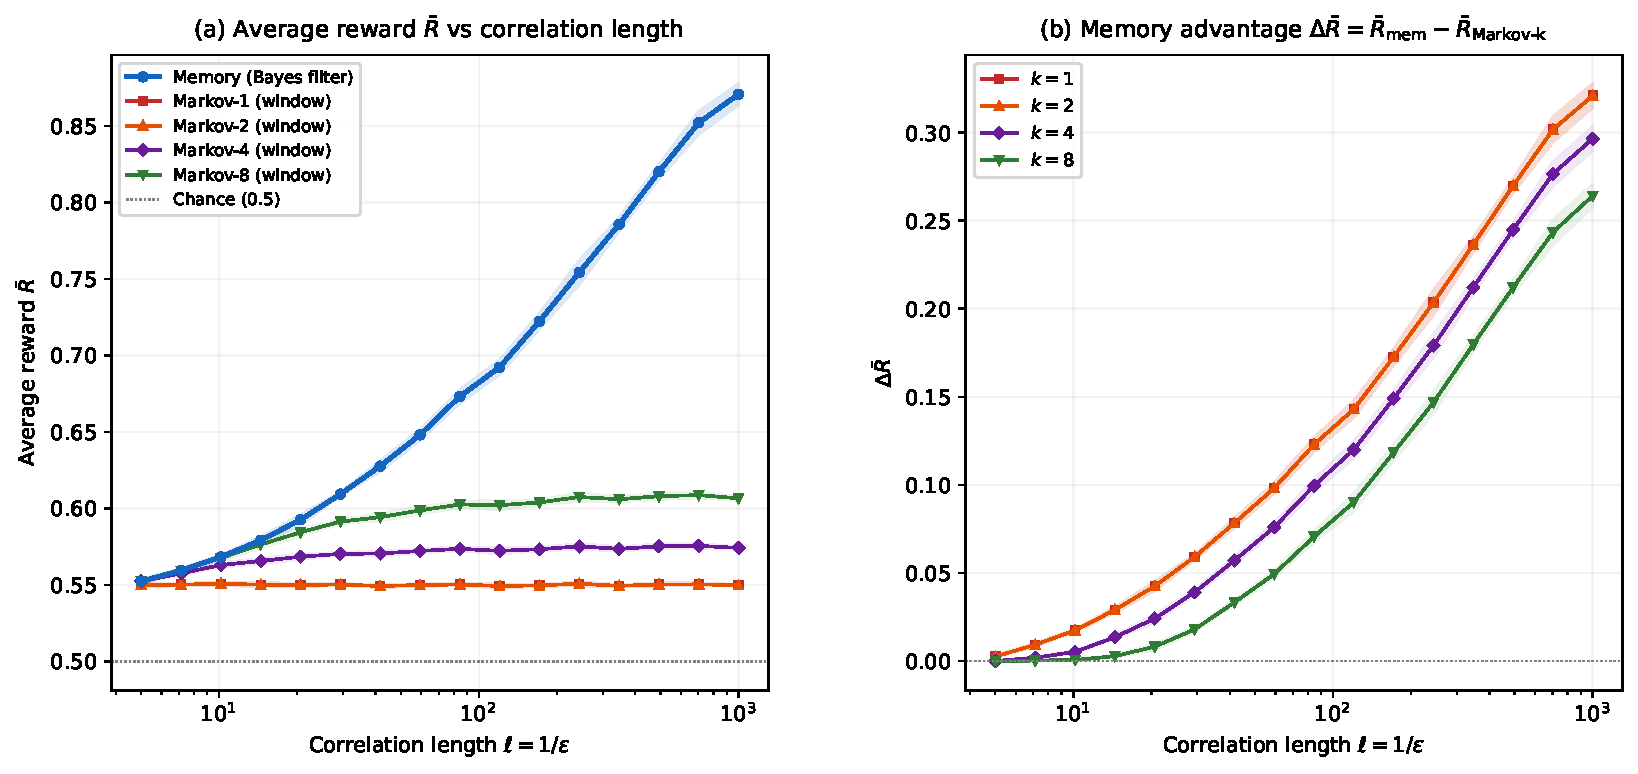
\includegraphics[width=\textwidth]{fig_paper1_markov_ceiling.pdf}
\caption{%
\textbf{Finite-window saturation and Bayes-filter advantage.}
Historical sweep: $T=10^5$ total steps, $2000$ discarded, 10 seeds. Shading uses $1.96$ times the across-seed standard deviation (with NumPy's population convention) divided by $\sqrt{10}$; these are normal-approximation error bands, not rigorous finite-sample confidence intervals.
\textbf{(a)}~Average reward $\bar R$ against correlation length $\ell=1/\varepsilon$. The Bayes filter (blue, bold) rises monotonically; Markov-$k$ agents saturate at $k$-dependent levels.
\textbf{(b)}~Gap $\Delta\bar R=\bar R_{\mathrm{mem}}-\bar R_{\mathrm{Markov}\text{-}k}$, which increases with $\ell$ and is larger for smaller $k$.}
\label{fig:markov_ceiling}
\end{figure}

The reward of the Bayes filter increases with the correlation length, while each Markov-$k$ agent saturates at a level ordered by $k$, all below the filter for $\ell\gtrsim20$ (Figure~\ref{fig:markov_ceiling}). The Markov-1 and Markov-2 curves nearly coincide at small $\ell$ because short windows add little in this aliasing regime. The sampled long-correlation regime shows an advantage over the four specified windows. For the given model and observation history, the full posterior Bayes decision minimizes classification risk. The example does not establish tight saturation constants or superiority across different reading and resource menus. Theorem~\ref{thm:value} supplies the conversion to work for a different task, in which the retained statistic is used for feedback on a system whose state it predicts. The supplementary source record gives the script, historical sweep and legacy-data distinction; these classification data do not computationally verify a survival-functional theorem.

% ============================================================
\section{Discussion}
\label{sec:discussion}

\subsection{The memory--self--introspection route}

In the task of Section~\ref{sec:value}, a work gain requires a memory carrying the relevant correlation. A protocol matched to its posterior realizes the value $k_BT\,I(X{:}M)$; every error in that posterior has a computable price. Reference calibration builds the required readout model, and reuse pays its preparation cost through the square-root amortization rule. Paper~III proves the stated scalar Gaussian drift law. These are the concrete links in the series' memory--self--introspection route. Proposition~\ref{prop:cycle} adds the reset condition for its allowed menu, and Proposition~\ref{prop:mixed_task} realizes positive task value with two partially mixed records. A useful second record reduces the reset price; a full apparatus cycle still has to renew the source, recording stock and bath supply. The conditions belong to this task and its allowed protocols. Driven Markovian systems can persist without memory or a self-model.

The results concern function. They show what an agent must hold and do to cash a record, and they do not show that holding a model of one's own readout is, or produces, experience. The relation between such functional self-models and first-person organization is treated in the Consciousness series with its own arguments.

The task fixes the record source, pointer basis and feedback device. Paper~II addresses how an agent selects what it reads; Paper~III addresses detection, the price of tracking, and repair selected by the history of its body-gated access. The three correlation models here remain distinct: the Lorentz--Drude bath carries pointer information without designated fragments, the two-qubit environment carries none, and collision records have no autonomous recurrence. Paper~III combines the collision records, a bounded changing instrument, a field-coupled actuator, harvest and reset on one ledger~\cite{Liu2026TDOME_III}. It exhibits a positive operating margin after body upkeep under supplied food, record purity, drive preparation, phase reference and timing. The calculation does not make those inputs products of the loop. Paper~III also constructs a continuing finite joint filter: a bounded changing instrument and controlled body generate the history that revises their model, with a uniform quantization-risk bound and adaptive reference timing. The updating mechanism is thus explicit under its stated transition law and resource permissions. Its processor, reference supply and drive preparation still need one sustainable apparatus ledger.

% ============================================================
\begin{thebibliography}{99}

\bibitem{BreuerPetruccione2002}
H.-P.~Breuer and F.~Petruccione,
\emph{The Theory of Open Quantum Systems},
Oxford University Press (2002).

\bibitem{Schrodinger1944}
E.~Schr\"odinger,
\emph{What is Life?},
Cambridge University Press (1944).

\bibitem{Lindblad1976}
G.~Lindblad,
\emph{On the generators of quantum dynamical semigroups},
Commun.\ Math.\ Phys.\ \textbf{48}, 119 (1976).

\bibitem{GKS1976}
V.~Gorini, A.~Kossakowski, and E.~C.~G.~Sudarshan,
\emph{Completely positive dynamical semigroups of $N$-level systems},
J.\ Math.\ Phys.\ \textbf{17}, 821 (1976).

\bibitem{Nakajima1958}
S.~Nakajima,
\emph{On quantum theory of transport phenomena},
Prog.\ Theor.\ Phys.\ \textbf{20}, 948 (1958).

\bibitem{Zwanzig1960}
R.~Zwanzig,
\emph{Ensemble method in the theory of irreversibility},
J.\ Chem.\ Phys.\ \textbf{33}, 1338 (1960).

\bibitem{SagawaUeda2008}
T.~Sagawa and M.~Ueda,
\emph{Second law of thermodynamics with discrete quantum feedback control},
Phys.\ Rev.\ Lett.\ \textbf{100}, 080403 (2008).

\bibitem{SagawaUeda2010}
T.~Sagawa and M.~Ueda,
\emph{Generalized Jarzynski Equality under Nonequilibrium Feedback Control},
Phys.\ Rev.\ Lett.\ \textbf{104}, 090602 (2010).

\bibitem{SagawaUeda2012}
T.~Sagawa and M.~Ueda,
\emph{Fluctuation Theorem with Information Exchange},
Phys.\ Rev.\ Lett.\ \textbf{109}, 180602 (2012).

\bibitem{RivasHuelgaPlenio2014}
\'{A}.~Rivas, S.~F.~Huelga, and M.~B.~Plenio,
\emph{Quantum non-Markovianity: characterization, quantification and detection},
Rep.\ Prog.\ Phys.\ \textbf{77}, 094001 (2014).

\bibitem{Spohn1978}
H.~Spohn,
\emph{Entropy production for quantum dynamical semigroups},
J.\ Math.\ Phys.\ \textbf{19}, 1227 (1978).

\bibitem{Landauer1961}
R.~Landauer,
\emph{Irreversibility and heat generation in the computing process},
IBM J.\ Res.\ Dev.\ \textbf{5}, 183 (1961).

\bibitem{Bennett1982}
C.~H.~Bennett,
\emph{The thermodynamics of computation---a review},
Int.\ J.\ Theor.\ Phys.\ \textbf{21}, 905 (1982).

\bibitem{BreuerLainePiilo2009}
H.-P.~Breuer, E.-M.~Laine, and J.~Piilo,
\emph{Measure for the Degree of Non-Markovian Behavior of Quantum Processes in Open Systems},
Phys.\ Rev.\ Lett.\ \textbf{103}, 210401 (2009).

\bibitem{EspositoLindenbergVandenBroeck2010}
M.~Esposito, K.~Lindenberg, and C.~Van~den~Broeck,
\emph{Entropy production as correlation between system and reservoir},
New J.\ Phys.\ \textbf{12}, 013013 (2010).

\bibitem{Wilde2017}
M.~M.~Wilde,
\emph{Quantum Information Theory}, 2nd ed.,
Cambridge University Press (2017).

\bibitem{SchallerAblassmayer2020}
G.~Schaller and J.~Abla{\ss}mayer,
\emph{Thermodynamics of the coarse-graining master equation},
Entropy \textbf{22}, 525 (2020); arXiv:2004.01554.

\bibitem{Holevo1973}
A.~S.~Holevo,
\emph{Bounds for the quantity of information transmitted by a quantum communication channel},
Probl.\ Inf.\ Transm.\ \textbf{9}, 177 (1973).

\bibitem{delRio2011}
L.~del Rio, J.~{\AA}berg, R.~Renner, O.~Dahlsten, and V.~Vedral,
\emph{The thermodynamic meaning of negative entropy},
Nature \textbf{474}, 61 (2011).

\bibitem{KolchinskyWolpert2017}
A.~Kolchinsky and D.~H.~Wolpert,
\emph{Dependence of dissipation on the initial distribution over states},
J.\ Stat.\ Mech.\ (2017) 083202.

\bibitem{ReebWolf2014}
D.~Reeb and M.~M.~Wolf,
\emph{An improved Landauer principle with finite-size corrections},
New J.\ Phys.\ \textbf{16}, 103011 (2014).

\bibitem{CrutchfieldFeldman2003}
J.~P.~Crutchfield and D.~P.~Feldman,
\emph{Regularities unseen, randomness observed: Levels of entropy convergence},
Chaos \textbf{13}, 25 (2003).

\bibitem{ShaliziCrutchfield2001}
C.~R.~Shalizi and J.~P.~Crutchfield,
\emph{Computational mechanics: Pattern and prediction, structure and simplicity},
J.\ Stat.\ Phys.\ \textbf{104}, 817 (2001).

\bibitem{BialekNemenmanTishby2001}
W.~Bialek, I.~Nemenman, and N.~Tishby,
\emph{Predictability, complexity, and learning},
Neural Computation \textbf{13}, 2409 (2001).

\bibitem{Liu2026HAFF_E}
S.~Liu, \emph{Measurement as Accessibility: Measurement Permissions, Stable Records and Public Readout} (HAFF~E), 2026; July record DOI: 10.5281/zenodo.18400065.

\bibitem{Liu2026HAFF_F}
S.~Liu, \emph{Records, Dissipation and Intervention: Conditions for a Temporal Direction} (HAFF~F), 2026; July record DOI: 10.5281/zenodo.18400425.

\bibitem{Liu2026QRAIF_B}
S.~Liu, \emph{Thermodynamic Stability Constraints on Persistent Open Quantum Subsystems: Control Algebra, Physical Actuation and Energy Cost}, Zenodo (2026), DOI: 10.5281/zenodo.18525890.

\bibitem{Liu2026TDOME_II}
S.~Liu, \emph{Reference Frames Selected by History: The Capability and Cost of a Bounded Agent's Self-Frame} (T-DOME~II), 2026; July record DOI: 10.5281/zenodo.18579703.

\bibitem{Liu2026TDOME_III}
S.~Liu, \emph{Keeping a Self-Model Calibrated: Drift Detection, the Price of Keeping Up, and Reliability in a Closed Loop} (T-DOME~III), 2026; July record DOI: 10.5281/zenodo.18591771.

\bibitem{Liu2026CIII}
S.~Liu, \emph{Finite Self-Models and the Explanatory Gap: What a Continuing Observer Can Know About Itself}, (2026), series record DOI: 10.5281/zenodo.19607724.

\bibitem{Hoeffding1963}
W.~Hoeffding,
\emph{Probability inequalities for sums of bounded random variables},
J.~Amer.~Statist.~Assoc.~\textbf{58}(301), 13--30 (1963),
DOI: 10.1080/01621459.1963.10500830.

\end{thebibliography}

\end{document}


